\newpage
\section*{Obvod}

Vstupy nášho obvodu sú generované čítačom:\\
a,Takto približne vyzeral čítač v simulátore Digital\\
\begin{center}
    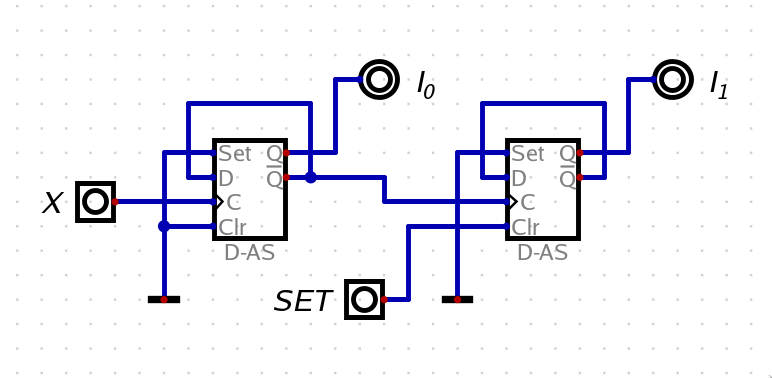
\includegraphics[width=16.2cm, height=7.2cm]{images/counter_dig.png}
\end{center}
b,Pri návrhu PCB boli potrebné aj negácie a preto sme ich začali využívať.
\begin{center}
    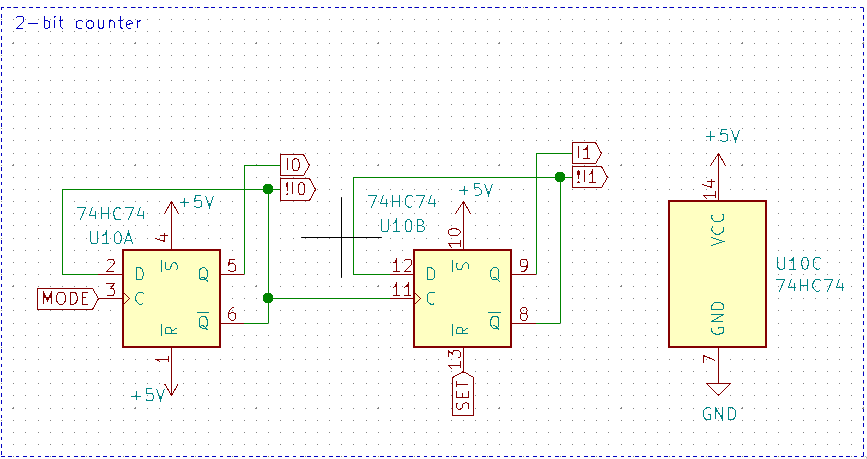
\includegraphics[width=16.2cm, height=8.5cm]{images/counter_kic.png}	
\end{center}

\newpage
\noindent
Synchronizačný signál bol generovaný časovačom 555\\
\begin{center}
    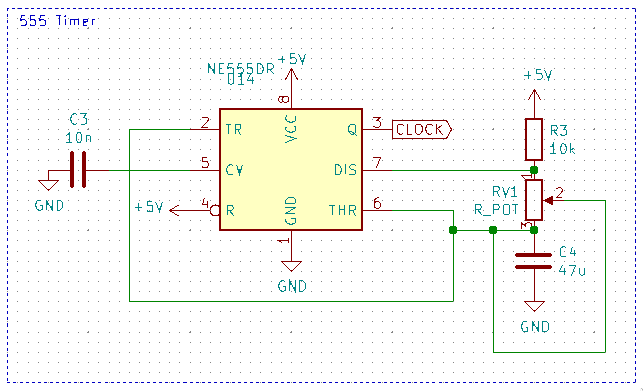
\includegraphics[width=16.2cm, height=9.6cm]{images/timer.png}
\end{center}

\newpage
\noindent
Dve tlačítka ovládajúce tento obvod:\\
\noindent
a, tlačítko slúžiace na nastavenie prvého stavu sekvenčného obvodu:
\begin{center}
    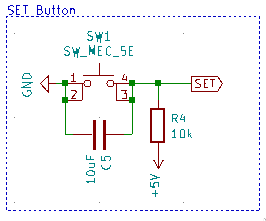
\includegraphics{images/sw1.png}
\end{center}
\noindent
b, tlačítko slúžiace na manipulovanie vstupov sekvenčného obvodu:
\begin{center}
    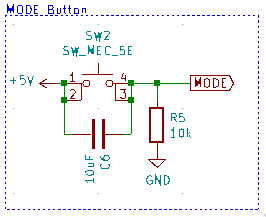
\includegraphics{images/sw2.png}
\end{center}


\newpage
\noindent
Samotný sekvenčný obvod v simulátore Digital a veľmi zjednodušená schéma celého obvodu:\\
\begin{center}
    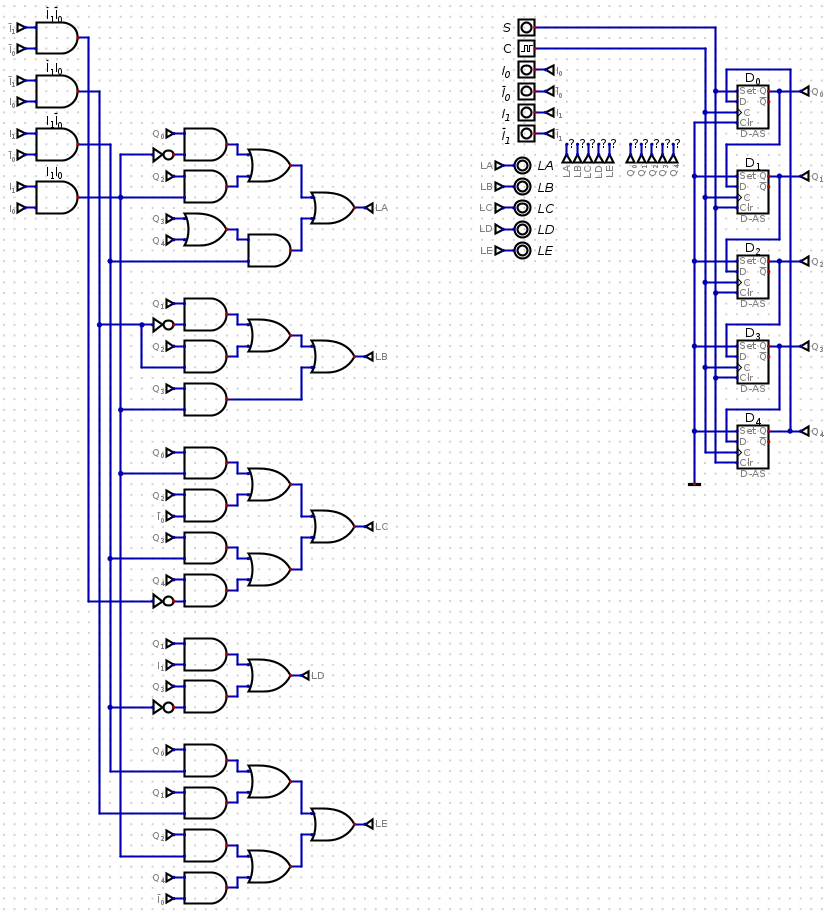
\includegraphics[width=16.2cm, height=17.8cm]{images/seq_dig.png}
\end{center}

\begin{center}
    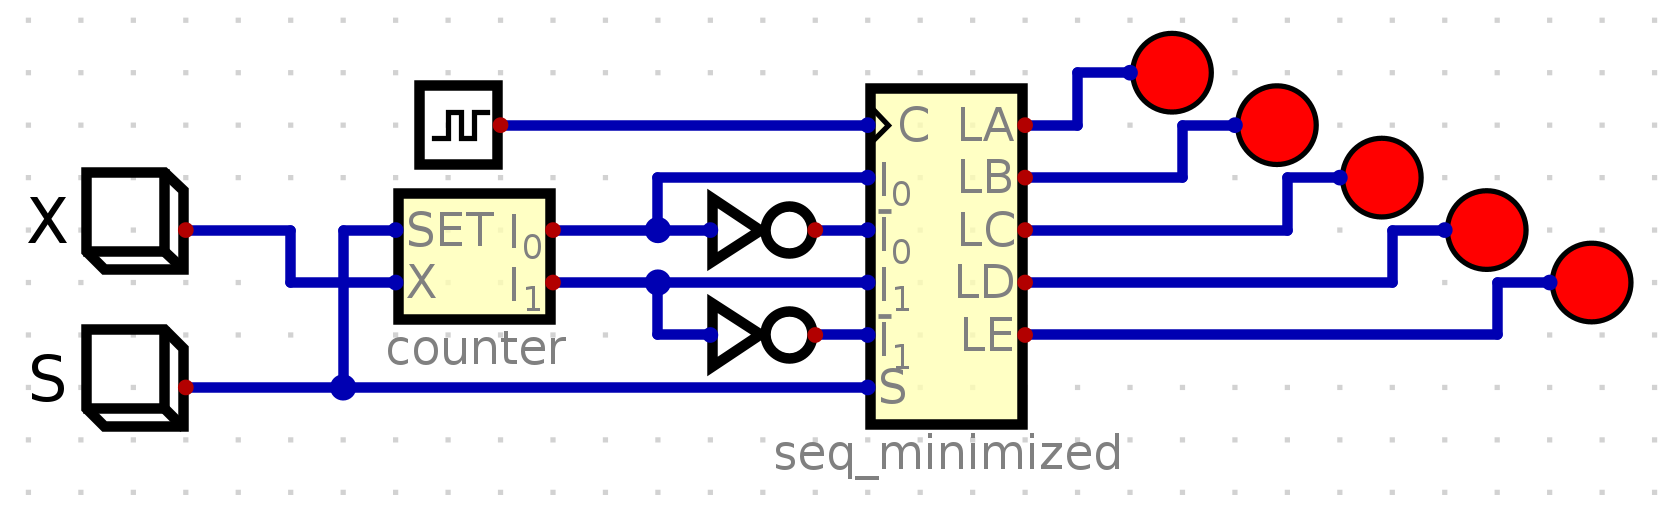
\includegraphics[width=16.2cm, height=5.04cm]{images/scheme-dig.png}
\end{center}

\newpage
\noindent
Schéma celého obvodu
\begin{center}
    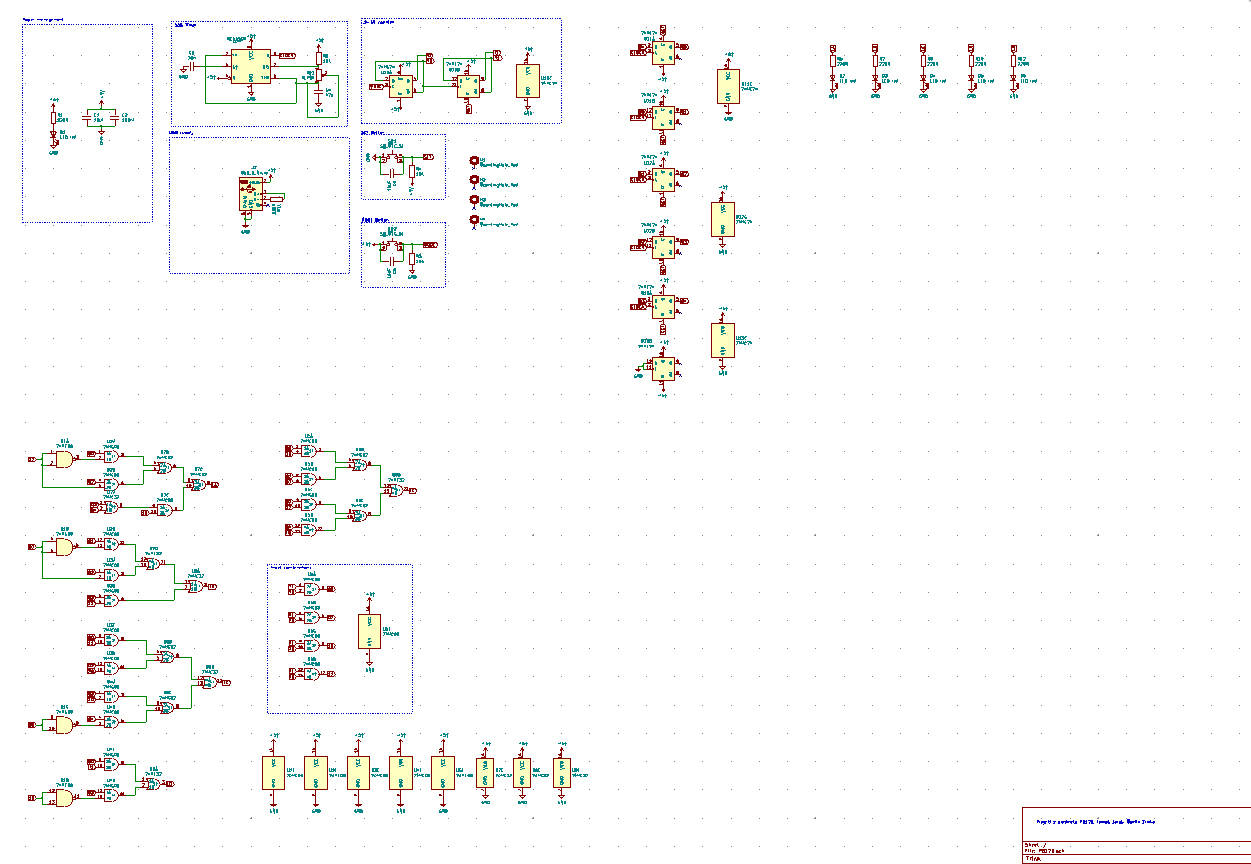
\includegraphics[width=16.2cm, height=10.32cm]{images/kicad.png}
\end{center}
Schéma napájania, časovača, čítača a tlačítok.
\begin{center}
    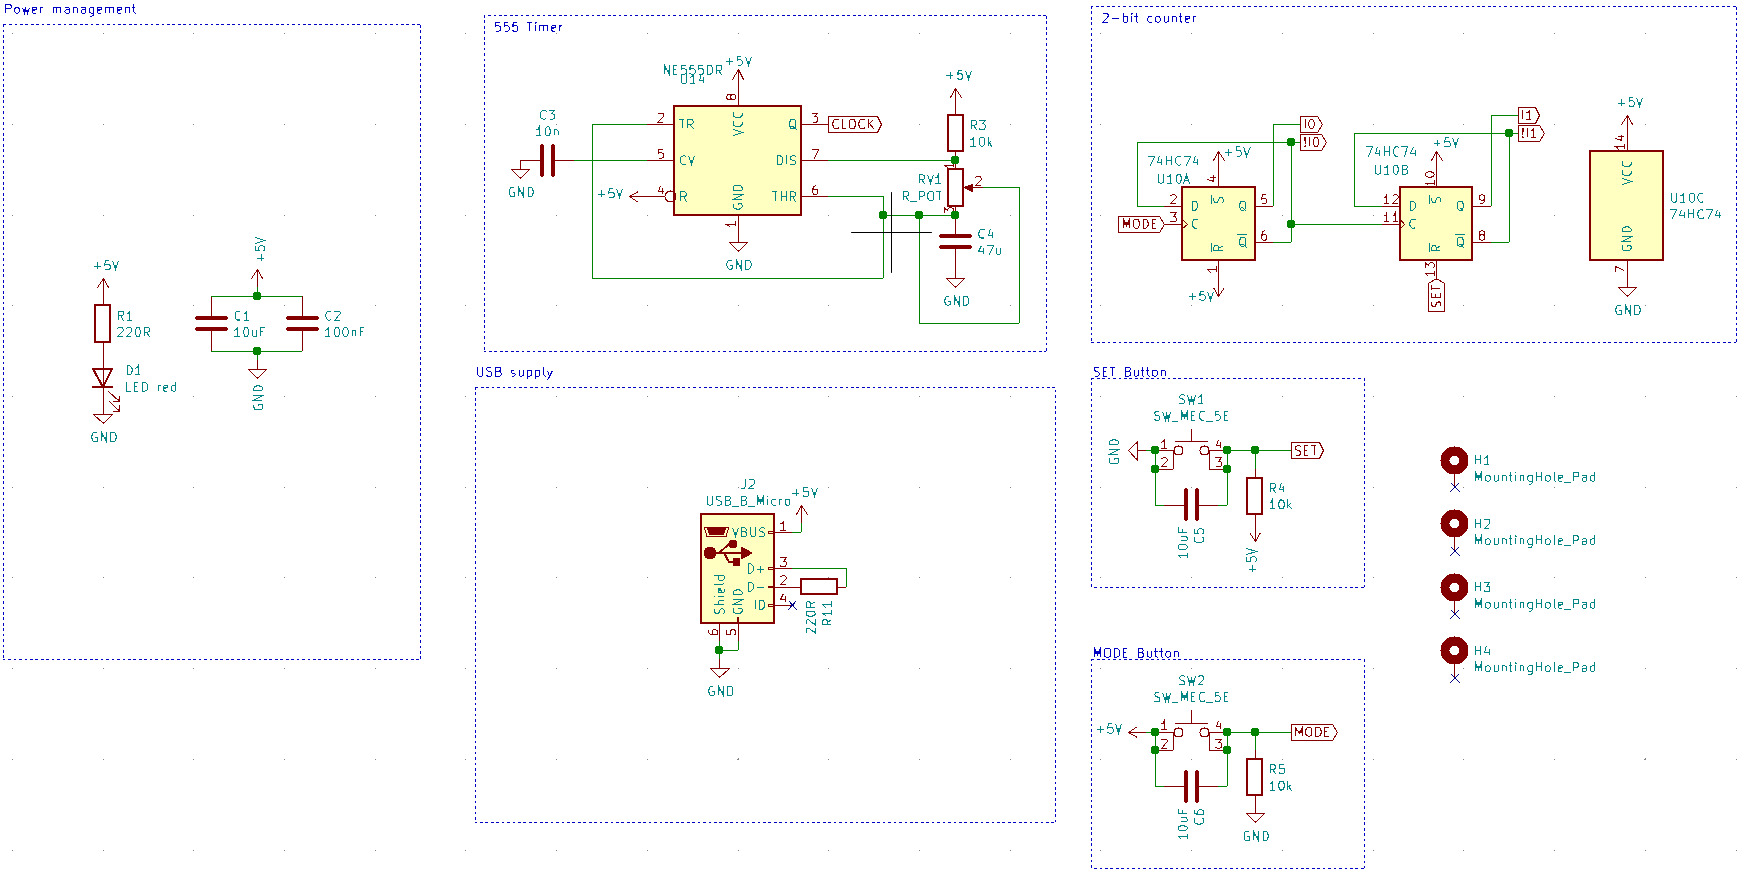
\includegraphics[width=16.2cm, height=8.1cm]{images/kicad2.png}
\end{center}
\newpage
\noindent
Časť s klopnými obvodmi a LEDkami.
\begin{center}
    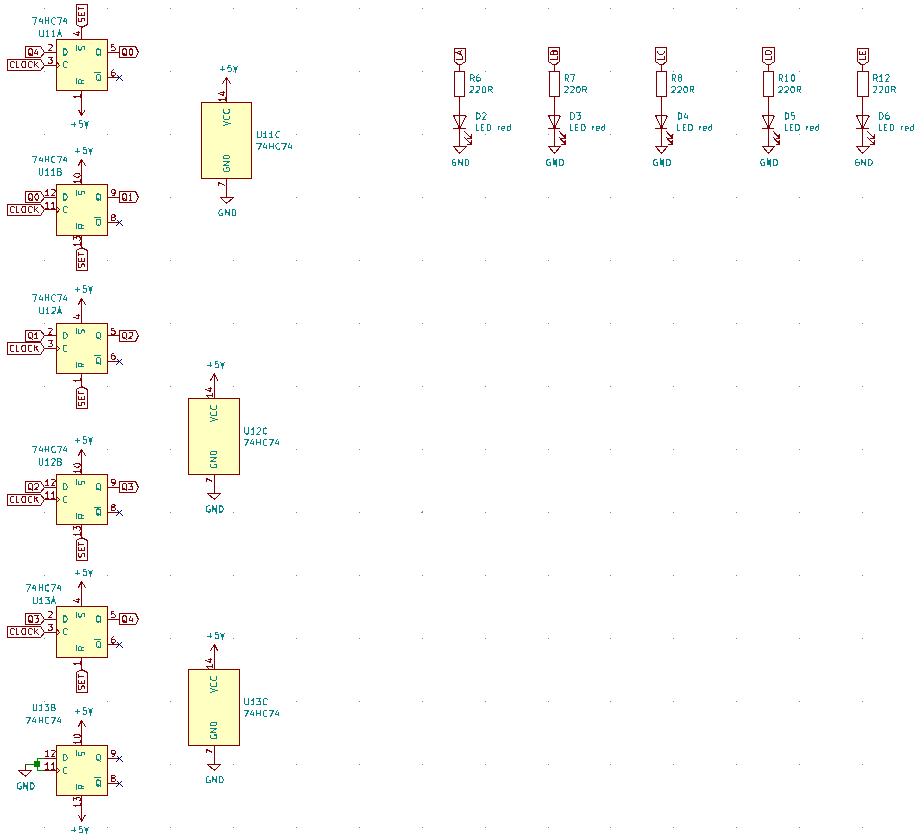
\includegraphics[width=16.2cm, height=14.7cm]{images/kicad3.png}
\end{center} 
\newpage
\noindent
Logická časť obvodu.
\begin{center}
    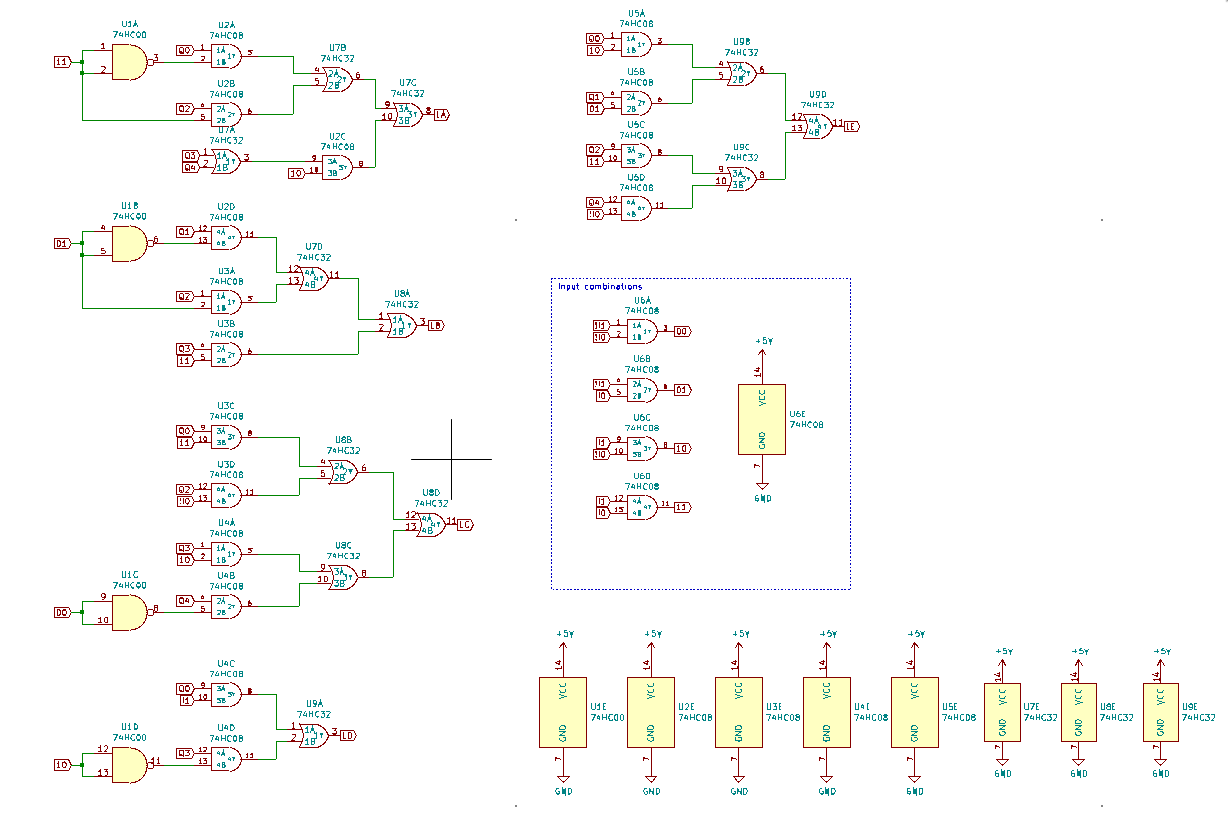
\includegraphics[width=16.2cm, height=11cm]{images/logic_kic.png}
\end{center}
Prikladáme model výslednej PCB dosky.
\begin{center}
    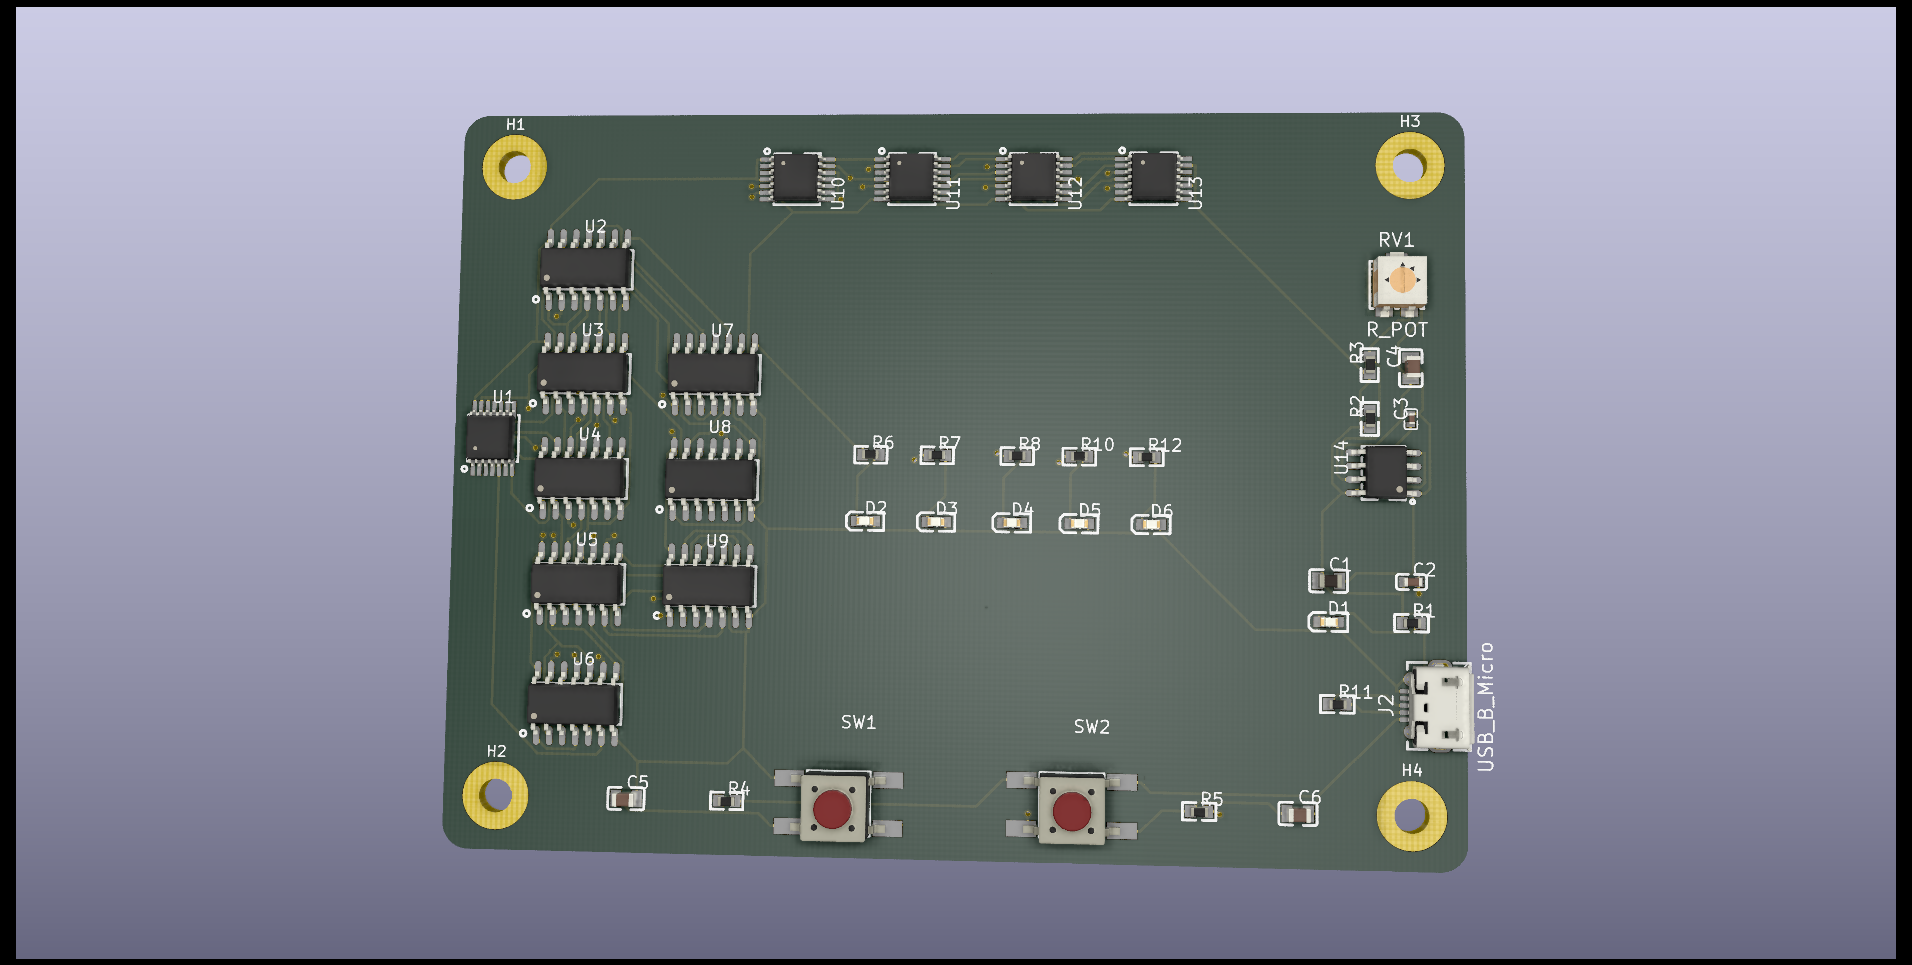
\includegraphics[width=17cm, height=8.4cm]{images/PB170.png}
\end{center}








